\section{Data management}

The data architecture is organized into the following key components:
\begin{enumerate}
    \item \textit{Source layer}: origin of raw data, which comes from operational systems, websites, e-commerce platforms, and other sources.
    \item \textit{Data ingestion}: data undergoes transformations to make it usable within the data platform. 
        This step ensures proper formatting for analysis, enabling businesses to derive value from the data.
    \item \textit{Data platform}: this is where core data analysis occurs. 
        Given the large volume of data, robust systems are essential for effective processing. 
        The data refinement process follows a tiered approach:
        \begin{itemize}
            \item \textit{Bronze layer}: raw ingested data.
            \item \textit{Silver layer}: data undergoes ETL processing.
            \item \textit{Gold layer}: fully analyzed and user-friendly data, optimized for reporting and decision-making.
        \end{itemize}
    \item \textit{Machine Learning} (optional): advanced analytics and machine learning techniques are applied to extract valuable insights and patterns from the processed data.
    \item \textit{Data consumer}: processed data and insights are delivered to end users or integrated into other applications.
\end{enumerate}

\begin{figure}[H]
    \centering
    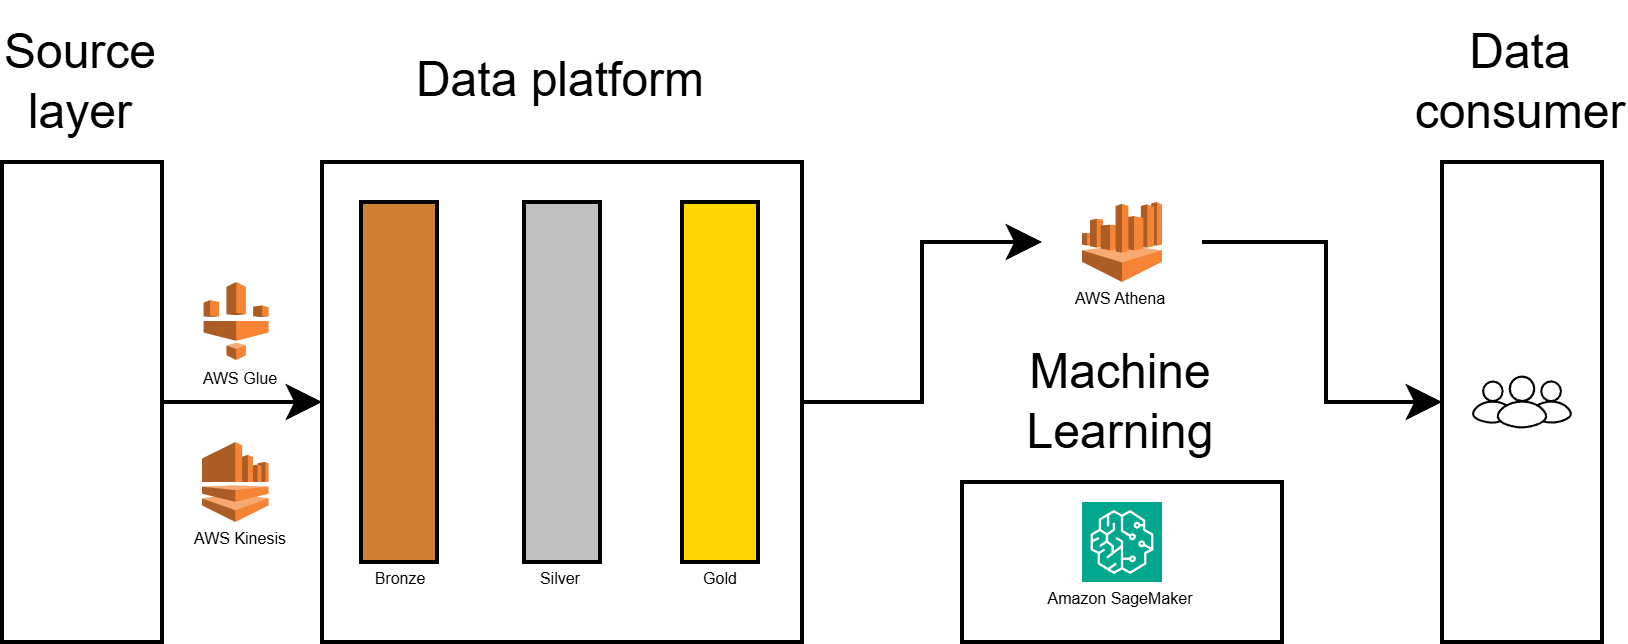
\includegraphics[width=0.75\linewidth]{images/bis11.png}
    \caption{Data architecture}
\end{figure}

\subsection{Data architecture}
A data architecture defines how data is managed throughout its lifecycle, from collection and transformation to distribution and consumption. 
It serves as a blueprint for how data flows through various storage systems, ensuring efficient processing and delivery.

In traditional data architectures, the Extract, Transform, Load (ETL) model is used. 
This method involves extracting data from sources, transforming it into a usable format, and loading it into a data warehouse for storage and analysis.

Modern data architectures, however, have shifted to the Extract, Load, Transform (ELT) approach. 
Instead of transforming all data before storage, raw data is directly placed in a data lake. From there, it can be analyzed as needed.
This approach offers greater flexibility and enables real-time analytics, allowing organizations to process and analyze data dynamically without waiting for full transformation.

\subsubsection{Data storage}
\begin{definition}[\textit{Data warehouse}]
    A data warehouse is a centralized repository that stores large volumes of structured data from various sources within an organization.
\end{definition}
\noindent Unlike transactional databases, which prioritize real-time operations, data warehouses are designed for analytical queries and historical data analysis. 
They facilitate reporting, business intelligence, and decision-making by providing a consolidated and structured view of organizational data.
\begin{definition}[\textit{Data lake}]
    A data lake is a scalable repository that allows organizations to store vast amounts of raw, structured, semi-structured, and unstructured data.
\end{definition}
\noindent Unlike a data warehouse, a data lake does not impose a schema on the data upon ingestion. 
Instead, it retains data in its original format until it is needed for processing or analysis.
While data lakes provide flexibility for advanced analytics and machine learning, they require careful governance and security measures to maintain data quality.

\begin{definition}[\textit{Data lakehouse}]
    A data lakehouse combines the strengths of data warehouses and data lakes.
\end{definition}
\noindent Data lakehouse integrates data warehouses and data lakes as part of a comprehensive data strategy, leveraging their respective advantages:
\begin{itemize}
    \item \textit{Data integration}: raw data is ingested into the data lake, preserving its original format and serving as a staging area before further processing.
    \item \textit{Data transformation}: ETL processes can occur in both the data lake and the data warehouse. 
        Structured data required for immediate reporting is transformed and stored in the warehouse, while raw and unstructured data remains in the lake for exploratory analysis.
\end{itemize}

\begin{definition}[\textit{Polyglot persistence}]
    Polyglot persistence refers to the practice of using multiple types of data storage technologies and databases within a single system.
\end{definition}
\noindent Instead of relying on a single storage solution, organizations select the best-suited technology for each specific data type and use case, optimizing performance and scalability across different applications.

\begin{definition}[\textit{Data mesh}]
    Data mesh is a modern approach to analytical data architecture that treats data as a product.
\end{definition}
\noindent It is domain-driven, meaning data ownership is distributed among teams with the best understanding of their data and its usage.
The key idea behind data mesh is that no one understands data better than its owner. Instead of relying on a centralized data team, data mesh distributes data responsibilities to domain-specific teams. 
Each domain aligns with a business function rather than specific applications or systems. 
Domains manage their own data pipelines within a shared infrastructure and provide access to domain-specific data and functionalities via APIs.

\renewcommand{\arraystretch}{1.5}
\begin{table}[!ht]
    \centering

    \begin{tabular}{|l|p{4cm}|p{4cm}|p{4cm}|}
        \hline
        \textbf{Feature} & \textbf{Data warehouse} & \textbf{Data lake} & \textbf{Data mesh} \\ \hline
        \textit{Centralization} & Centralized & Centralized & Decentralized \\ \hline
        \textit{Data structure} & Structured & Unstructured & Both \\ \hline
        \textit{Use cases} & Reporting & Advanced analytics & Data product \\ \hline
        \textit{Integration} & Data lake & Data warehouse & Autonomous \\ \hline
        \textit{Flexibility} & No & No & Yes \\ \hline
    \end{tabular}
\end{table}
\renewcommand{\arraystretch}{1}

\subsubsection{Data modeling}
\begin{definition}[\textit{Data modeling}]
    Data modeling refers to the process of creating a structured representation of data to analyze its relationships, constraints, and organization. 
\end{definition}
\noindent Data modeling plays a critical role in structuring data to guide database design and enable smooth, reliable operations. 
It involves defining entities, their attributes, and the connections between them within a database. 
By doing so, it provides a blueprint that supports efficient data management and retrieval.

Data modeling encompasses various approaches and tools, including:
\begin{itemize}
    \item \textit{Data dictionaries}: comprehensive references that describe each data element within a system or database.
    \item \textit{Entity-relationship diagrams}: visual representations of relational databases, illustrating the relationships between entities.
    \item \textit{Semantic models}: logical layers containing transformations, calculations, and relationships between data sources, often used for creating reports and dashboards.
\end{itemize}
\noindent In data warehousing and business intelligence, data is typically categorized into two primary types:
\begin{itemize}
    \item \textit{Dimensions}: represent descriptive attributes or entities within the model.
    \item \textit{Facts}: store measurable, quantitative data related to specific observations or events.
\end{itemize}

Two fundamental approaches to organizing data in relational databases are normalization and denormalization. 
The choice between these methods depends on the application's requirements and objectives. 

\paragraph*{Normalization}
Normalization prioritizes data integrity by minimizing redundancy and \\ avoiding anomalies. 
It is particularly suitable for transactional databases where accuracy and consistency are paramount.

\paragraph*{Denormalization}
Denormalization focuses on optimizing query performance, especially for read-heavy workloads or reporting databases.
 While it introduces some level of redundancy, it significantly enhances query execution speed.

\subsubsection{Data visualization}
Data visualization offers an intuitive way to explore and analyze data by transforming raw numbers into meaningful graphical insights. 
It serves as a powerful tool for uncovering hidden patterns, trends, and relationships that may not be evident through traditional analysis.

\paragraph*{Application}
Data visualization enables interactive exploration and graphical representation of data, regardless of dataset size or origin. 
It empowers managers and decision-makers to: identify key trends and outliers, gain actionable insights from complex datasets, and make informed, data-driven decisions.

\subsection{Data governance}
Data governance refers to the framework that defines how an organization manages its data to ensure accuracy, security, and compliance. 
It encompasses processes, roles, policies, standards, and metrics aimed at optimizing data usage, enabling organizations to become truly data-driven.
\begin{figure}[H]
    \centering
    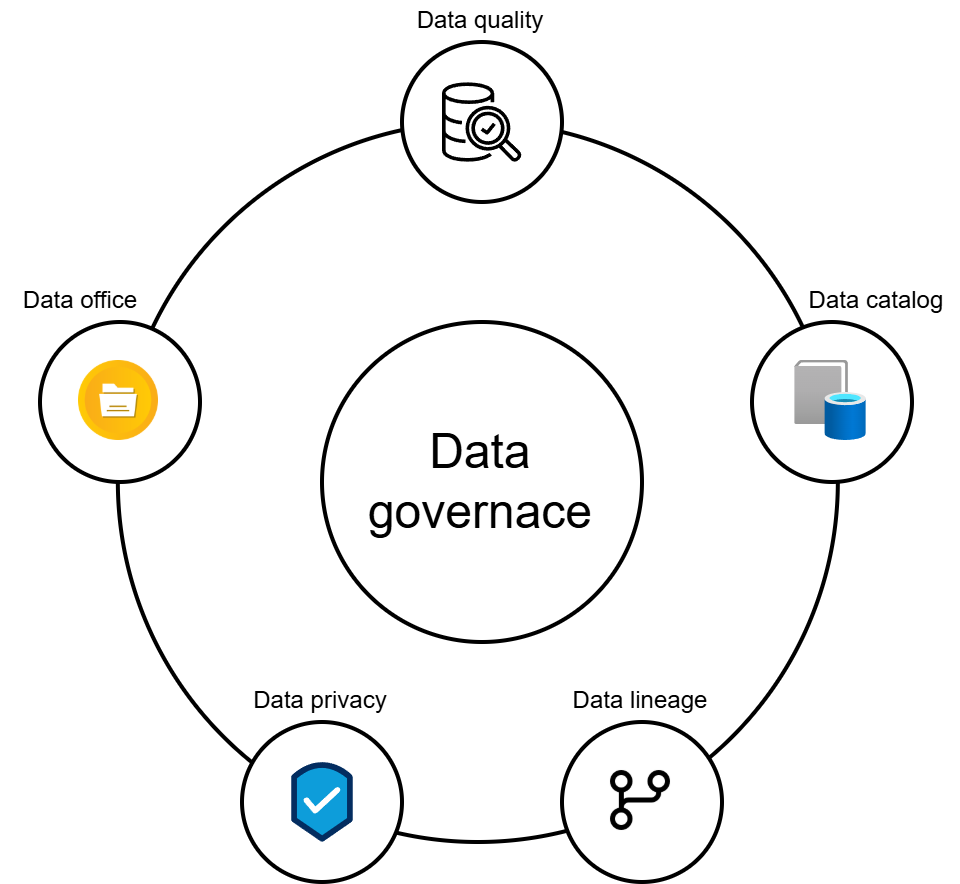
\includegraphics[width=0.5\linewidth]{images/bis12.png}
    \caption{Data governance pillars}
\end{figure}
Data governance is built on several key pillars that collectively ensure the integrity, usability, and protection of data assets:
\begin{itemize}
    \item \textit{Data quality}: ensures that information is accurate, reliable, and well-maintained throughout its lifecycle.
    \item \textit{Data catalog}: helps organizations manage and understand their data assets by integrating metadata from diverse sources, including databases, cloud platforms, ETL processes, and business intelligence tools.
    \item \textit{Data lineage}: tracks the entire lifecycle of data, from its origin to its final destination.
    \item \textit{Data privacy}: focuses on identifying and safeguarding sensitive information. 
    \item \textit{Data office}: plays a central role in overseeing data governance initiatives.
\end{itemize}
\noindent Organizations rely on specialized technology platforms to implement robust data governance strategies. 
These tools provide comprehensive capabilities for: managing data quality, cataloging metadata, tracking data lineage, and ensuring data privacy. 
However, technology alone is insufficient. 
Effective governance requires a combination of tools, processes, and dedicated personnel within a structured data office to ensure alignment with organizational goals.

Beyond compliance and data management, data governance serves as a strategic enabler for organizations. 
By establishing strong governance practices, companies can achieve data as a service and data monetization.